% !TEX program = pdflatex
\documentclass[11pt,a4paper]{article}

\usepackage[T1]{fontenc}
\usepackage[utf8]{inputenc}
\IfFileExists{lmodern.sty}{\usepackage{lmodern}\usepackage{microtype}}{\usepackage[expansion=false]{microtype}}
\usepackage[a4paper,left=22mm,right=22mm,top=27mm,bottom=22mm,headheight=22pt]{geometry}
\usepackage[table]{xcolor}
\usepackage{array,longtable,booktabs}
\usepackage{enumitem}
\usepackage{titlesec}
\usepackage{fancyhdr}
\usepackage[most]{tcolorbox}
\usepackage[hyphens]{url}
\usepackage[colorlinks=true,linkcolor=accent,urlcolor=accent,citecolor=accent,pdfusetitle,bookmarksnumbered,pageanchor=false]{hyperref}
\usepackage{tikz}
\usetikzlibrary{arrows.meta,positioning,shapes.geometric,calc,fit,backgrounds}

% ---------- palette ----------
\definecolor{ink}{HTML}{16202B}
\definecolor{accent}{HTML}{2458A6}
\definecolor{muted}{HTML}{4A5563}
\definecolor{rulec}{HTML}{CBD3DC}
\definecolor{shade}{HTML}{EEF2F6}
\definecolor{headbg}{HTML}{DCE6F2}
\definecolor{green}{HTML}{16A34A}
\definecolor{amber}{HTML}{D97706}
\definecolor{red}{HTML}{DC2626}

% ---------- headings ----------
\titleformat{\section}{\sffamily\Large\bfseries\color{accent}}{\thesection.}{0.5em}{}
\titleformat{\subsection}{\sffamily\large\bfseries\color{ink}}{\thesubsection}{0.6em}{}
\titleformat{\subsubsection}{\sffamily\normalsize\bfseries\color{ink}}{}{0em}{}
\titlespacing*{\section}{0pt}{16pt}{8pt}
\titlespacing*{\subsection}{0pt}{11pt}{5pt}

% ---------- header / footer ----------
\pagestyle{fancy}
\fancyhf{}
\fancyhead[L]{\sffamily\footnotesize\color{muted}Plan de Estudio --- CI+SIL \texttimes{} zz\_Workflow}
\fancyhead[R]{\sffamily\footnotesize\color{muted}v2.0 --- October 2026}
\fancyfoot[C]{\sffamily\footnotesize\thepage}
\renewcommand{\headrulewidth}{0.4pt}
\renewcommand{\headrule}{\hbox to\headwidth{\color{rulec}\leaders\hrule height \headrulewidth\hfill}}

% ---------- body ----------
\setlength{\parindent}{0pt}
\setlength{\parskip}{5pt}
\setlist{itemsep=2pt,topsep=3pt}
\renewcommand{\arraystretch}{1.25}

% ---------- custom boxes ----------
\newtcolorbox{notebox}{enhanced,colback=shade,colframe=accent,boxrule=0pt,leftrule=3pt,sharp corners,
  left=8pt,right=8pt,top=6pt,bottom=6pt,fontupper=\itshape}

\newtcolorbox{goalbox}[1][]{enhanced,colback=shade,colframe=green!80!black,boxrule=0pt,leftrule=3pt,sharp corners,
  left=8pt,right=8pt,top=6pt,bottom=6pt,title={\sffamily\bfseries\color{green!80!black}#1}}

\newtcolorbox{questionbox}[1][]{enhanced,colback=shade,colframe=accent,boxrule=0pt,leftrule=3pt,sharp corners,
  left=8pt,right=8pt,top=6pt,bottom=6pt,title={\sffamily\bfseries\color{accent}#1}}

\newtcolorbox{deliverbox}[1][]{enhanced,colback=shade,colframe=amber!80!black,boxrule=0pt,leftrule=3pt,sharp corners,
  left=8pt,right=8pt,top=6pt,bottom=6pt,title={\sffamily\bfseries\color{amber!80!black}#1}}

\newcommand{\timeest}[1]{\textsf{\footnotesize\color{muted}#1}}

\hypersetup{pdftitle={Plan de Estudio Conceptual: CI+SIL x zz\_Workflow},pdfsubject={Conceptual study plan},pdfauthor={David Ram\'irez-Betancourt}}

\begin{document}
\begin{titlepage}
\thispagestyle{empty}
\noindent\colorbox{accent}{\makebox[\dimexpr\textwidth-2\fboxsep][l]{\rule{0pt}{4pt}}}
\vspace*{30mm}

{\sffamily\bfseries\color{muted} AI-Assisted SDR Design --- Methodology Study\par}
\vspace{4mm}
{\raggedright\hyphenpenalty=10000\exhyphenpenalty=10000\sffamily\bfseries\fontsize{26}{31}\selectfont\color{ink} Plan de Estudio Conceptual\par}
\vspace{2mm}
{\raggedright\sffamily\bfseries\fontsize{18}{22}\selectfont\color{accent} CI+SIL \texttimes{} zz\_Workflow\par}
\vspace{5mm}
{\large\color{muted} Ruta de aprendizaje para comprender en profundidad los conceptos, principios y decisiones de dise\~no detr\'as de la metodolog\'ia de verificaci\'on continua acoplada al motor de prototipado asistido por LLM.\par}
\vspace{14mm}
{\small\begin{tabular}{@{}>{\bfseries\sffamily\raggedright\arraybackslash}p{0.2\textwidth}>{\raggedright\arraybackslash}p{0.74\textwidth}@{}}
Autor & David Ram\'irez-Betancourt \\[3pt]
Afiliaci\'on & Universidad Nacional de Colombia --- GCPDS \\[3pt]
Fecha & Octubre 2026 \\[3pt]
Enfoque & Conceptual --- sin c\'odigo ni matem\'aticas \\[3pt]
Tiempo total & $\sim$4 semanas (ritmo medio: 6--8 h/semana) \\[3pt]
Prerequisitos & Curiosidad y ganas de leer con atenci\'on \\
\end{tabular}}

\vfill
\begin{notebox}
\textbf{C\'omo usar este plan.} Cada m\'odulo tiene: una pregunta central que lo gu\'ia, lecturas con secciones espec\'ificas, preguntas de reflexi\'on, y un entregable escrito. Los m\'odulos se construyen uno sobre otro. No hay c\'odigo ni f\'ormulas: el foco est\'a en entender el \textbf{por qu\'e} de cada decisi\'on de dise\~no.
\end{notebox}
\end{titlepage}

\newpage

% ---------- Roadmap visual ----------
\section{Mapa de la Ruta}

\begin{center}
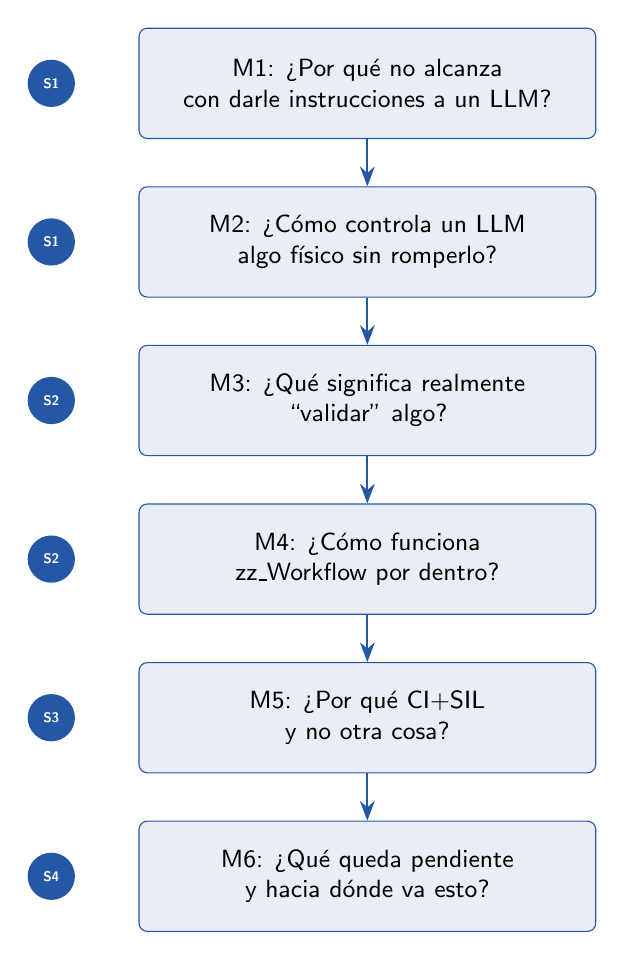
\begin{tikzpicture}[
  node distance=6mm and 10mm,
  stage/.style={rectangle, rounded corners=3pt, draw=accent, fill=accent!10,
    minimum height=14mm, minimum width=58mm, font=\sffamily\small, align=center},
  question/.style={font=\itshape\scriptsize\color{muted}, text width=55mm, align=left},
  week/.style={circle, fill=accent, text=white, font=\sffamily\tiny\bfseries,
    minimum size=6mm, inner sep=0pt},
  arr/.style={-{Stealth[length=2.5mm]}, thick, accent},
]
  \node[stage] (m1) {M1: ?`Por qu\'e no alcanza\\con darle instrucciones a un LLM?};
  \node[stage, below=of m1] (m2) {M2: ?`C\'omo controla un LLM\\algo f\'isico sin romperlo?};
  \node[stage, below=of m2] (m3) {M3: ?`Qu\'e significa realmente\\``validar'' algo?};
  \node[stage, below=of m3] (m4) {M4: ?`C\'omo funciona\\zz\_Workflow por dentro?};
  \node[stage, below=of m4] (m5) {M5: ?`Por qu\'e CI+SIL\\y no otra cosa?};
  \node[stage, below=of m5] (m6) {M6: ?`Qu\'e queda pendiente\\y hacia d\'onde va esto?};

  \node[week, left=8mm of m1] {S1};
  \node[week, left=8mm of m2] {S1};
  \node[week, left=8mm of m3] {S2};
  \node[week, left=8mm of m4] {S2};
  \node[week, left=8mm of m5] {S3};
  \node[week, left=8mm of m6] {S4};

  \draw[arr] (m1) -- (m2);
  \draw[arr] (m2) -- (m3);
  \draw[arr] (m3) -- (m4);
  \draw[arr] (m4) -- (m5);
  \draw[arr] (m5) -- (m6);
\end{tikzpicture}
\end{center}

% ============================================================
\section{M\'odulo 1: ?`Por qu\'e no alcanza con darle instrucciones a un LLM?}
\timeest{Semana 1, primera mitad --- 4 h}

\begin{goalbox}[Pregunta central]
Si un LLM puede generar c\'odigo, dise\~nar arquitecturas y razonar sobre problemas complejos, ?`por qu\'e necesita una estructura r\'igida alrededor? ?`Qu\'e sale mal cuando lo dej\'as solo?
\end{goalbox}

\subsection{Ideas clave a entender}
\begin{itemize}
  \item \textbf{El LLM es probabil\'istico.} Incluso a temperatura cero, hay una ``temperatura de fondo'' que hace que dos ejecuciones id\'enticas puedan dar resultados distintos. La repetibilidad no se puede \textit{asumir}; hay que \textit{medir}.
  \item \textbf{Se degrada en cadenas largas.} Cuando un agente ejecuta muchos pasos secuenciales, la probabilidad de \'exito cae r\'apidamente. Hay un techo pr\'actico de $\sim$16 pasos antes de que todos los modelos colapsen. La implicaci\'on: los stages tienen que ser cortos y acotados.
  \item \textbf{Los m\'etricos de accuracy incentivan mentir.} Si el benchmark castiga ``no s\'e'' tanto como una respuesta incorrecta, el modelo aprende a adivinar con confianza en lugar de abstenerse. Consecuencia: la auto-evaluaci\'on del modelo no es confiable.
  \item \textbf{Estructura > instrucciones.} Ponerle m\'as texto al prompt no mejora la confiabilidad tanto como darle interfaces tipadas, loops de verificaci\'on y gates expl\'icitos. El contexto (qu\'e ve el modelo en cada paso) importa m\'as que c\'omo se lo ped\'is.
\end{itemize}

\subsection{Lecturas}
\begin{enumerate}[label=\textbf{L\arabic*.}]
  \item Mittal, ``How Fast Do Agents Rot?,'' arXiv:2609.01660 --- \S1--3.
  \item Kalai et al., ``Evaluating LLMs for accuracy incentivizes hallucinations,'' \textit{Nature} 653, 2026 --- abstract y \S2.
  \item Anthropic, ``Effective context engineering for AI agents,'' 2026 --- completo.
\end{enumerate}

\subsection{Preguntas de reflexi\'on}
\begin{enumerate}[label=\textbf{R\arabic*.}]
  \item Si un modelo tiene 97\% de \'exito por paso, ?`por qu\'e eso no es suficiente para una cadena de 20 pasos? Explicar la intuici\'on sin f\'ormulas.
  \item ?`Qu\'e significa ``structure beats instructions''? Dar una analog\'ia de la vida cotidiana (ejemplo: sem\'aforo vs.\ cartel de ``maneje con cuidado'').
  \item Si el modelo incentiva adivinar en vez de decir ``no s\'e'', ?`podemos confiar en que \'el mismo nos diga cu\'ando se equivoc\'o?
\end{enumerate}

\begin{deliverbox}[Entregable]
Escrito de 1 p\'agina: ``Por qu\'e un LLM necesita estructura externa'' --- explicado como si se lo contaras a un colega que nunca us\'o un agente de IA.
\end{deliverbox}

% ============================================================
\section{M\'odulo 2: ?`C\'omo controla un LLM algo f\'isico sin romperlo?}
\timeest{Semana 1, segunda mitad --- 4 h}

\begin{goalbox}[Pregunta central]
Un LLM solo produce texto. ?`C\'omo llega ese texto a mover una antena, cambiar una frecuencia o encender un transmisor? ?`Qu\'e pasa si se equivoca?
\end{goalbox}

\subsection{Ideas clave a entender}
\begin{itemize}
  \item \textbf{Tools como manos del agente.} El LLM no toca el hardware directamente. Llama a \textit{tools} (funciones con par\'ametros tipados) a trav\'es de un protocolo (MCP). El tool traduce la intenci\'on del LLM en una acci\'on f\'isica.
  \item \textbf{El lazo cerrado.} Agente $\to$ Tool $\to$ Actuador $\to$ Planta f\'isica $\to$ Sensor $\to$ feedback al agente. Sin este feedback, el agente opera a ciegas.
  \item \textbf{Control de dos niveles.} El LLM piensa lento y planifica; un controlador determin\'istico ejecuta el lazo r\'apido. El LLM \textbf{nunca} est\'a en el fast loop --- ser\'ia demasiado lento e impredecible.
  \item \textbf{Dos barreras humanas distintas:}
    \begin{itemize}
      \item \textbf{HITL} (Human in the Loop) = barrera de \textit{autorizaci\'on}. ``?`Puedo hacer esto?''
      \item \textbf{HIL} (Hardware in the Loop) = barrera de \textit{validaci\'on}. ``?`Esto funciona en el hardware real?''
    \end{itemize}
  \item \textbf{L\'imites f\'isicos en el esquema.} Si el tool define que la frecuencia m\'axima es 1766\,MHz, una llamada con 2000\,MHz se rechaza \textit{antes} de llegar al hardware. Es la primera defensa.
\end{itemize}

\subsection{Lecturas}
\begin{enumerate}[label=\textbf{L\arabic*.}]
  \item MCP Specification rev.\ 2025-06-18 --- \url{modelcontextprotocol.io} --- secci\'on ``Architecture'' y ``Tools''.
  \item Sadeqi Bajestani et al., ``HITL+LLM in smart manufacturing,'' \textit{J.\ Manufacturing Systems} 86, 2026 --- \S1 y \S3.
  \item ``LLMs Add Safety Risks to Physical AI,'' SemiEngineering, Nov.\ 2025 --- completo (incluye el caso del robot de ajedrez que le fractur\'o un dedo a un ni\~no).
\end{enumerate}

\subsection{Preguntas de reflexi\'on}
\begin{enumerate}[label=\textbf{R\arabic*.}]
  \item ?`Por qu\'e el LLM no puede estar en el fast loop de un controlador? Pensar en t\'erminos de velocidad de respuesta y predictibilidad.
  \item Explicar la diferencia entre HITL y HIL con un ejemplo concreto del proyecto SDR.
  \item Si un agente puede llamar 50 tools distintos, ?`eso lo hace m\'as capaz o m\'as peligroso? ?`C\'omo se mitiga?
\end{enumerate}

\begin{deliverbox}[Entregable]
Diagrama dibujado a mano (o en cualquier herramienta) del lazo cerrado agente--hardware, marcando d\'onde entra HITL, d\'onde entra HIL, y d\'onde est\'an los l\'imites f\'isicos del schema. A\~nadir 3 oraciones explicando por qu\'e el LLM planifica pero no ejecuta.
\end{deliverbox}

% ============================================================
\section{M\'odulo 3: ?`Qu\'e significa realmente ``validar'' algo?}
\timeest{Semana 2, primera mitad --- 4 h}

\begin{goalbox}[Pregunta central]
Todo el mundo dice ``hay que validar''. Pero, ?`validar contra qu\'e? ?`Qui\'en decide si pas\'o? ?`Es lo mismo verificar que validar?
\end{goalbox}

\subsection{Ideas clave a entender}
\begin{itemize}
  \item \textbf{Verificar $\neq$ validar.}
    \begin{itemize}
      \item \textit{Verificaci\'on}: ``?`Lo constru\'i bien?'' --- el producto cumple su especificaci\'on interna.
      \item \textit{Validaci\'on}: ``?`Constru\'i lo correcto?'' --- el producto resuelve el problema real del usuario.
    \end{itemize}
  \item \textbf{Nadie valida en un solo paso.} Se valida en capas que van de lo barato a lo caro: primero en software, despu\'es en simulaci\'on, despu\'es en hardware, despu\'es con humanos.
  \item \textbf{El oracle no puede ser el generador.} Si el mismo componente que genera la respuesta tambi\'en la eval\'ua, la presi\'on de optimizaci\'on explota las debilidades del evaluador, no mejora la respuesta real.
  \item \textbf{El humano act\'ua en los extremos.} Al principio (encuadre del problema) y al final (juicio experto). En el medio, los chequeos deben ser lo m\'as autom\'aticos y determin\'isticos posible.
  \item \textbf{Cinco enfoques conocidos:}
    \begin{enumerate}
      \item V-model: trazabilidad requisito $\leftrightarrow$ test.
      \item CI+SIL: regresi\'on autom\'atica en software simulado.
      \item Bancos HIL: hardware real en el lazo.
      \item LLM-as-judge + HITL: el modelo eval\'ua, el humano arbitra.
      \item MCDA: decisi\'on multi-criterio para elegir entre alternativas.
    \end{enumerate}
  \item \textbf{El flujo de 6 fases} organiza estos enfoques en secuencia: Encuadre $\to$ Modelo $\to$ Software/CI $\to$ Banco HIL $\to$ Juicio $\to$ Decisi\'on MCDA, con gates entre cada fase.
\end{itemize}

\subsection{Lecturas}
\begin{enumerate}[label=\textbf{L\arabic*.}]
  \item Sheridan Tech, ``Design Validation vs Verification,'' Mar.\ 2026 --- completo.
  \item OPAL-RT, ``Guide to HIL Testing,'' Sep.\ 2026 --- \S1--3 (qu\'e es, cu\'ando usarlo).
  \item ``Autonomous Research Agents: Verification Gap,'' arXiv:2608.05179 --- completo (el 83\% publica c\'odigo, pero solo el 38\% da artefactos reproducibles).
\end{enumerate}

\subsection{Preguntas de reflexi\'on}
\begin{enumerate}[label=\textbf{R\arabic*.}]
  \item Explicar con una analog\'ia de construcci\'on de una casa la diferencia entre verificar y validar.
  \item ?`Por qu\'e el oracle no puede ser el generador? Imaginar que un estudiante se pone su propia nota --- ?`qu\'e incentivos tiene?
  \item ?`Por qu\'e validar en capas de barato a caro es m\'as eficiente que ir directo al test m\'as completo?
  \item De las 6 fases, ?`cu\'al es la m\'as barata de ejecutar? ?`Cu\'al es la m\'as cara? ?`Por qu\'e est\'an en ese orden?
\end{enumerate}

\begin{deliverbox}[Entregable]
Diagrama del flujo de 6 fases con los gates, incluyendo para cada fase: qui\'en es el oracle y qu\'e pregunta responde. M\'as un p\'arrafo sobre ``verificar vs.\ validar'' en tus propias palabras.
\end{deliverbox}

% ============================================================
\section{M\'odulo 4: ?`C\'omo funciona zz\_Workflow por dentro?}
\timeest{Semana 2, segunda mitad --- 4 h}

\begin{goalbox}[Pregunta central]
zz\_Workflow es el motor que produce prototipos verificados. ?`C\'omo est\'a organizado internamente? ?`Qu\'e reglas lo gobiernan? ?`Qu\'e produce y qu\'e NO produce?
\end{goalbox}

\subsection{Ideas clave a entender}
\begin{itemize}
  \item \textbf{4 stages acotados} (Ctx 00--03), cada uno con un contexto espec\'ifico:
    \begin{itemize}
      \item Ctx 00: Definir el problema y congelar el alcance.
      \item Ctx 01: Fijar requisitos y criterios de aceptaci\'on.
      \item Ctx 02: Elegir la arquitectura y el plan de implementaci\'on.
      \item Ctx 03: Contrato de implementaci\'on (qu\'e entra, qu\'e sale, qu\'e restricciones tiene).
    \end{itemize}
  \item \textbf{Gates humanas.} Entre cada stage hay un humano que decide si se avanza. El modelo \textbf{redacta} pero \textbf{nunca aprueba} su propia salida.
  \item \textbf{La regla de oro:} ``La aceptaci\'on se decide por criterios pre-declarados aplicados a mediciones registradas, nunca por juicio del modelo.''
  \item \textbf{6 artefactos gobernantes} que definen c\'omo opera el workflow:
    \begin{enumerate}
      \item Mapa de arquitectura de prompts.
      \item Especificaciones de RAG (qu\'e documentos alimentan al modelo).
      \item \textbf{Suites de evaluaci\'on y benchmarking} --- el Artefacto 3, que corre chequeos de regresi\'on despu\'es de cualquier cambio.
      \item Guardrails (reglas determin\'isticas que el modelo no puede violar).
      \item Telemetr\'ia (registro de qu\'e pas\'o, qu\'e fall\'o y por qu\'e).
      \item Privacidad y gobernanza.
    \end{enumerate}
  \item \textbf{Routing de defectos R0--R3.} Cuando algo falla, no se dice simplemente ``fall\'o''. Se clasifica el defecto y se devuelve al stage responsable:
    \begin{itemize}
      \item R0 $\to$ el problema estaba mal definido (volver a Ctx 00).
      \item R1 $\to$ los requisitos estaban incompletos (volver a Ctx 01).
      \item R2 $\to$ la arquitectura era inadecuada (volver a Ctx 02).
      \item R3 $\to$ la implementaci\'on tiene un bug (volver a Ctx 03).
    \end{itemize}
  \item \textbf{Salida terminal:} Prototipo Verificado + Evidencia. Es expl\'icitamente \textit{verificaci\'on}, no validaci\'on. El workflow es honesto sobre lo que entrega.
\end{itemize}

\subsection{Lecturas}
\begin{enumerate}[label=\textbf{L\arabic*.}]
  \item \texttt{context/golden\_ctx\_CI-SIL\_+\_zz/zz\_Workflow\_.md} --- completo, es el documento fuente.
  \item Takahara \& Mizoguchi, ``Toward Auditable AI Scientists,'' arXiv:2607.09195 --- \S1--2 (por qu\'e importa la auditabilidad).
\end{enumerate}

\subsection{Preguntas de reflexi\'on}
\begin{enumerate}[label=\textbf{R\arabic*.}]
  \item ?`Por qu\'e los stages son ``acotados por contexto'' en vez de ser etapas libres? ?`Qu\'e problema resuelve acotar lo que el modelo ve en cada momento?
  \item Explicar la regla de oro con un ejemplo: si el modelo dice ``el detector funciona bien'', ?`por qu\'e eso no cuenta como aceptaci\'on?
  \item ?`Qu\'e diferencia hay entre decir ``el Pd fall\'o'' (sin routing) y decir ``R2: la arquitectura es inadecuada, volver a Ctx 02''? ?`Por qu\'e el segundo es m\'as \'util?
  \item El workflow produce un \textit{Prototipo Verificado}. ?`Qu\'e falta para que sea un \textit{Prototipo Validado}? ?`Qui\'en o qu\'e proporciona esa pieza faltante?
\end{enumerate}

\begin{deliverbox}[Entregable]
Diagrama de zz\_Workflow con los 4 stages, las gates humanas, los 6 artefactos, y las rutas R0--R3. A\~nadir una nota al pie del diagrama: ``Produce verificaci\'on, no validaci\'on --- y eso es intencional.''
\end{deliverbox}

% ============================================================
\section{M\'odulo 5: ?`Por qu\'e CI+SIL y no otra cosa?}
\timeest{Semana 3 --- 8 h}

\begin{goalbox}[Pregunta central]
Hay 5 metodolog\'ias de validaci\'on disponibles. ?`Por qu\'e CI+SIL es el acople natural con zz\_Workflow? ?`Qu\'e hace que el ajuste sea ``HIGH/clean'' y no forzado?
\end{goalbox}

\subsection{Ideas clave a entender}
\begin{itemize}
  \item \textbf{El Artefacto 3 ya ES un harness de regresi\'on.} No hay que inventar nada nuevo. Las suites de evaluaci\'on que zz\_Workflow ya requiere son exactamente lo que CI necesita ejecutar. El acople es natural, no forzado.
  \item \textbf{El trigger no es solo un commit de c\'odigo.} En un sistema asistido por LLM, un cambio de modelo, de prompt o de contexto puede alterar el comportamiento sin tocar una sola l\'inea de c\'odigo. CI+SIL lo reconoce: el trigger es cualquier cambio en modelo, prompt o Ctx.
  \item \textbf{SIL = replay controlado.} Software-in-the-Loop significa que se reproducen se\~nales sint\'eticas (golden I/Q) sin usar RF real. Es barato, repetible y determin\'istico.
  \item \textbf{Omitir LLM-as-judge para aceptaci\'on es una fortaleza.} Cuando el mismo componente que propone tambi\'en eval\'ua, la optimizaci\'on converge hacia explotar las debilidades del evaluador. La receta: separaci\'on de roles + gates determin\'isticos donde ``el rechazo mec\'anico le gana a la aprobaci\'on del LLM, nunca al rev\'es''.
  \item \textbf{La coupling matrix:}

  \begin{center}
  \begin{tabular}{@{}lll@{}}
    \toprule
    \textbf{Metodolog\'ia} & \textbf{Acople} & \textbf{Raz\'on} \\
    \midrule
    CI+SIL & HIGH / clean & Artefacto 3 ya es el harness \\
    V\&V (V-model) & HIGH--MEDIUM & Compatible pero pesado \\
    LLM-judge + HITL & MEDIUM & \'Util para revisi\'on, no para aceptaci\'on \\
    Bancos HIL & MEDIUM--LOW & Necesita infraestructura f\'isica \\
    MCDA & LOW & Aplica a selecci\'on multi-hip\'otesis \\
    \bottomrule
  \end{tabular}
  \end{center}

  \item \textbf{Cobertura de las 6 fases:}
    \begin{itemize}
      \item Fases 1, 3, 5: \textbf{cubiertas} (encuadre, software/CI, juicio humano).
      \item Fase 2: \textbf{parcial} (hay arquitectura y golden I/Q, pero falta un modelo f\'isico predictivo independiente).
      \item Fases 4 y 6: \textbf{gaps} (HIL real y MCDA quedan downstream).
    \end{itemize}
\end{itemize}

\subsection{Lecturas}
\begin{enumerate}[label=\textbf{L\arabic*.}]
  \item \texttt{context/golden\_ctx\_CI-SIL\_+\_zz/Acople de zz\_Workflow.html} --- completo.
  \item ``LLM-as-a-Judge Is Not an Oracle,'' arXiv:2609.02246 --- completo.
  \item \texttt{context/golden\_ctx\_CI-SIL\_+\_zz/CI+SIL \texttimes{} zz\_Workflow.html} --- explorar los 3 tabs del diagrama interactivo.
\end{enumerate}

\subsection{Preguntas de reflexi\'on}
\begin{enumerate}[label=\textbf{R\arabic*.}]
  \item Explicar en tus palabras por qu\'e ``el Artefacto 3 ya es un CI harness'' es el argumento central del acople.
  \item ?`Por qu\'e el trigger de CI debe incluir cambios de prompt y modelo, no solo commits de c\'odigo? Dar un ejemplo donde un cambio de prompt rompe el comportamiento sin cambiar c\'odigo.
  \item Un colega propone usar LLM-as-judge para decidir si el prototipo pasa. ?`Qu\'e le responder\'ias y por qu\'e? Usar el argumento de arXiv:2609.02246.
  \item De los dos gaps (HIL y MCDA), ?`cu\'al es m\'as urgente de cerrar para el proyecto SDR y por qu\'e?
\end{enumerate}

\begin{deliverbox}[Entregable]
Ensayo de 2 p\'aginas: ``Por qu\'e CI+SIL es el primer tier de integraci\'on para zz\_Workflow'' --- incluir la coupling matrix, el argumento del Artefacto 3, la raz\'on para omitir LLM-as-judge, y los gaps pendientes.
\end{deliverbox}

% ============================================================
\section{M\'odulo 6: ?`Qu\'e queda pendiente y hacia d\'onde va esto?}
\timeest{Semana 4 --- 6 h}

\begin{goalbox}[Pregunta central]
CI+SIL cubre la verificaci\'on continua. Pero ``verificado'' no es ``validado''. ?`Qu\'e falta? ?`Cu\'al es el camino desde un prototipo verificado hasta uno validado?
\end{goalbox}

\subsection{Ideas clave a entender}
\begin{itemize}
  \item \textbf{``Verificado en simulaci\'on'' $\neq$ ``validado''.} El claim debe nombrar el ambiente en el que se produjo la evidencia. Un prototipo que pasa todos los tests con se\~nales sint\'eticas NO est\'a validado en hardware real.
  \item \textbf{Gap 1 --- Banco HIL.} Para ir de verificaci\'on a validaci\'on se necesita un banco de hardware in the loop: SDR real, se\~nales RF reales (o capturadas), y mediciones f\'isicas. Esto cierra la fase 4.
  \item \textbf{Gap 2 --- MCDA.} Cuando hay m\'ultiples hip\'otesis de dise\~no (distintas arquitecturas de detector, por ejemplo), se necesita un m\'etodo de decisi\'on multi-criterio para elegir entre ellas. Esto cierra la fase 6. No aplica mientras haya un solo prototipo.
  \item \textbf{Gap 2b --- Modelo f\'isico independiente.} La fase 2 es parcial porque no hay un modelo predictivo que act\'ue como oracle independiente del c\'odigo. Un modelo anal\'itico de propagaci\'on FM podr\'ia cerrar esto.
  \item \textbf{La honestidad del nombre.} Llamar al output ``Prototipo Verificado'' y no ``Prototipo Validado'' no es modestia: es precisi\'on. Mantener esta distinci\'on hace que los claims sean tractables y las pr\'oximas etapas est\'en claras.
\end{itemize}

\subsection{Lecturas}
\begin{enumerate}[label=\textbf{L\arabic*.}]
  \item Heinrichs et al., ``From Prompt to Prototype: LLM-Driven RF Workflow,'' arXiv:2608.31006 --- \S4--5 (gap entre simulaci\'on y fabricaci\'on/medici\'on).
  \item OPAL-RT, ``Guide to HIL Testing,'' Sep.\ 2026 --- \S4--6 (c\'omo montar un banco HIL).
  \item \textit{Sustainable Futures}, ``MCDA reliability,'' Jun.\ 2026 --- \S1--3 (cu\'ando usar y cu\'ando no usar MCDA).
\end{enumerate}

\subsection{Preguntas de reflexi\'on}
\begin{enumerate}[label=\textbf{R\arabic*.}]
  \item Dibujar la secuencia completa: zz\_Workflow $\to$ CI+SIL $\to$ Banco HIL $\to$ Validaci\'on. ?`D\'onde cambia el tipo de evidencia de ``sint\'etica'' a ``real''?
  \item ?`Por qu\'e es importante \textit{nombrar} la diferencia entre verificado y validado, en vez de usar los t\'erminos de forma intercambiable?
  \item Si tu proyecto tiene un solo dise\~no de detector, ?`necesit\'as MCDA? ?`Cu\'ando empezar\'ia a ser relevante?
  \item Imaginar que mont\'as el banco HIL y el detector falla con RF real pero pasaba en simulaci\'on. ?`A qu\'e ruta R lo devolver\'ias? ?`Por qu\'e?
\end{enumerate}

\begin{deliverbox}[Entregable final]
Mapa conceptual completo de la metodolog\'ia, desde los fundamentos de LLM hasta los gaps pendientes. Debe responder las 4 preguntas del criterio de completitud (ver abajo). Formato libre: mapa mental, diagrama, o texto estructurado.
\end{deliverbox}

% ============================================================
\section{Criterio de Completitud}

\begin{center}
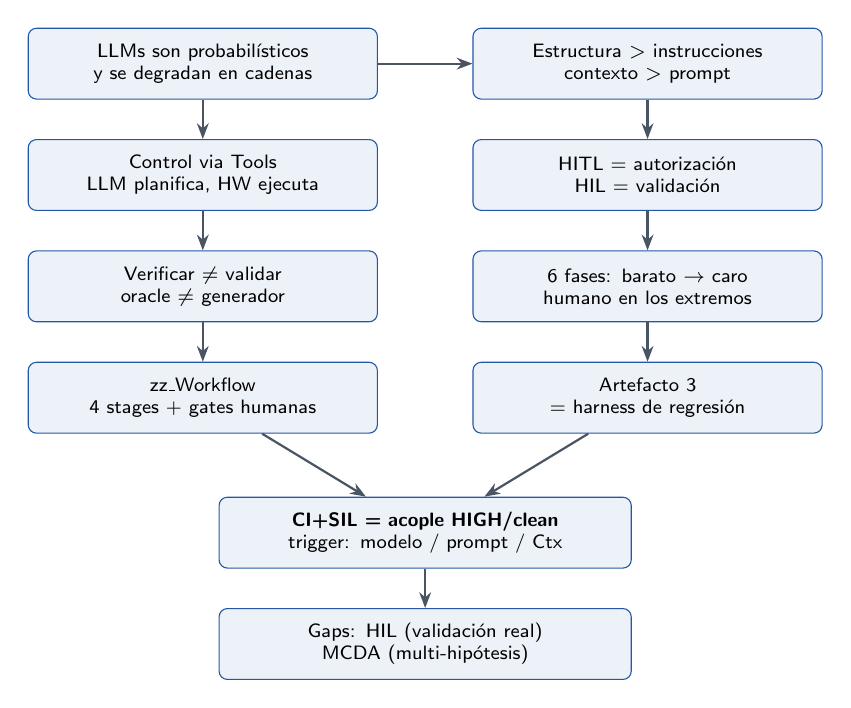
\begin{tikzpicture}[
  node distance=5mm and 8mm,
  concept/.style={rectangle, rounded corners=3pt, draw=accent, fill=accent!8,
    minimum height=9mm, text width=42mm, font=\sffamily\scriptsize, align=center},
  link/.style={-{Stealth[length=2mm]}, thick, muted},
]
  \node[concept] (prob) {LLMs son probabil\'isticos\\y se degradan en cadenas};
  \node[concept, right=12mm of prob] (struct) {Estructura $>$ instrucciones\\contexto $>$ prompt};
  \node[concept, below=of prob] (tools) {Control via Tools\\LLM planifica, HW ejecuta};
  \node[concept, below=of struct] (twolevel) {HITL = autorizaci\'on\\HIL = validaci\'on};
  \node[concept, below=of tools] (valid) {Verificar $\neq$ validar\\oracle $\neq$ generador};
  \node[concept, below=of twolevel] (sixphase) {6 fases: barato $\to$ caro\\humano en los extremos};
  \node[concept, below=of valid] (zz) {zz\_Workflow\\4 stages + gates humanas};
  \node[concept, below=of sixphase] (art3) {Artefacto 3\\= harness de regresi\'on};
  \node[concept, below=8mm of $(zz.south)!0.5!(art3.south)$, text width=50mm] (cisil) {\textbf{CI+SIL = acople HIGH/clean}\\trigger: modelo / prompt / Ctx};
  \node[concept, below=of cisil, text width=50mm] (gaps) {Gaps: HIL (validaci\'on real)\\MCDA (multi-hip\'otesis)};

  \draw[link] (prob) -- (struct);
  \draw[link] (prob) -- (tools);
  \draw[link] (struct) -- (twolevel);
  \draw[link] (tools) -- (valid);
  \draw[link] (twolevel) -- (sixphase);
  \draw[link] (valid) -- (zz);
  \draw[link] (sixphase) -- (art3);
  \draw[link] (zz) -- (cisil);
  \draw[link] (art3) -- (cisil);
  \draw[link] (cisil) -- (gaps);
\end{tikzpicture}
\end{center}

\vspace{8pt}

\begin{notebox}
\textbf{Sab\'es que dominaste la metodolog\'ia si pod\'es explicar a otro ingeniero:}
\begin{enumerate}
  \item Por qu\'e un LLM no puede auto-verificarse (el oracle no es el generador).
  \item Qu\'e produce zz\_Workflow (prototipo verificado + evidencia) y qu\'e NO produce (validaci\'on).
  \item Por qu\'e el Artefacto 3 ya es un CI harness (el acople no se inventa, se descubre).
  \item Qu\'e falta para ir de ``verificado'' a ``validado'' (HIL, modelo f\'isico independiente).
\end{enumerate}
\end{notebox}

\end{document}
